\documentclass[9pt,letterpaper]{article}

\usepackage[utf8]{inputenc}
\usepackage[spanish]{babel}
\usepackage{geometry}
\geometry{top=1.8cm, bottom=2cm, left=2cm, right=2cm}
\usepackage{helvet}
\renewcommand{\familydefault}{\sfdefault}
\usepackage{xcolor}
\definecolor{primary}{RGB}{0,102,68}
\definecolor{secondary}{RGB}{255,204,51}
\definecolor{lightgray}{RGB}{245,245,245}
\definecolor{textgray}{RGB}{80,80,80}
\usepackage{graphicx}
\usepackage{booktabs}
\usepackage{enumitem}
\usepackage[hidelinks]{hyperref}
\usepackage{multicol}
\usepackage{fancyhdr}
\pagestyle{fancy}
\fancyhf{}
\lhead{\footnotesize \textcolor{primary}{Microservicio BPO-AI --- Documento Técnico de Arquitectura}}
\rhead{\footnotesize \thepage}
\renewcommand{\headrulewidth}{0.2pt}
\usepackage{titlesec}
\titleformat{\section}
  {\normalsize\bfseries\color{primary}}
  {\thesection.}{0.4em}{}
\titleformat{\subsection}
  {\small\bfseries}
  {\thesubsection}{0.3em}{}
\setlength{\parskip}{3pt}
\setlength{\parindent}{0pt}
\usepackage{tcolorbox}
\tcbset{
  colback=lightgray,
  colframe=primary,
  boxrule=0.4pt,
  arc=3pt,
  left=4pt, right=4pt, top=4pt, bottom=4pt
}
\newtcolorbox{highlightbox}{
  colback=secondary!20,
  colframe=secondary,
  boxrule=0.5pt,
  arc=3pt,
  left=4pt, right=4pt, top=4pt, bottom=4pt
}

\begin{document}

{\large \textbf{Documento Técnico de Arquitectura}} \\[-2pt]
{\small Microservicio Transversal de IA --- Gestión de Solicitudes BPO}

\vspace{0.2cm}
\textbf{Autor:} Manuel Sebastián Torres Hernández \hfill \textbf{Fecha:} \today
\vspace{0.3cm}
\textcolor{primary}{\rule{\textwidth}{1pt}}
\vspace{-0.8cm}

% ── RESUMEN ──────────────────────────────────────────────────────────────────
\section{Resumen Ejecutivo}

El microservicio BPO-AI automatiza los pasos 1 al 6 del proceso de gestión de solicitudes: validación semántica, clasificación, asignación de prioridad, generación de justificación, decisión del siguiente paso y creación del caso en plataformas externas. Está diseñado para operar de forma transversal sobre múltiples empresas cliente, cada una con sus propias categorías, reglas de prioridad e integraciones.

\begin{highlightbox}
\textbf{Decisión estratégica:} Se adoptó un enfoque híbrido LLM + reglas de negocio configurables. El LLM gestiona la comprensión del lenguaje natural (validación, clasificación, justificación); las reglas deterministas del YAML controlan prioridad y enrutamiento. Esto garantiza interpretabilidad, auditabilidad y adaptabilidad por cliente sin depender del modelo para decisiones de negocio críticas.
\end{highlightbox}
\vspace{-0.2cm}
% ── ARQUITECTURA ─────────────────────────────────────────────────────────────
\section{Arquitectura de la Solución}

\subsection{Justificación del enfoque híbrido}

Un modelo puramente basado en reglas no puede manejar texto libre con variabilidad lingüística. Un LLM puro para prioridad y enrutamiento sería opaco, no auditable y susceptible a alucinaciones en decisiones de negocio. El enfoque híbrido asigna cada responsabilidad al mecanismo más adecuado:

\begin{center}
\small
\begin{tabular}{@{}lll@{}}
\toprule
\textbf{Paso} & \textbf{Mecanismo} & \textbf{Razón} \\
\midrule
Validación semántica & LLM & Comprende texto libre, extrae entidades \\
Clasificación & LLM + validación post-modelo & Entiende intención, pero se restringe a categorías del YAML \\
Prioridad & Reglas YAML / servicio externo & Auditable, determinístico, cambiable por cliente \\
Justificación & LLM & Redacción en lenguaje natural \\
Siguiente paso & Reglas YAML & Determinístico, contrato contractual con el cliente \\
Caso externo & Adaptador por empresa & Desacoplado de la lógica de negocio \\
\bottomrule
\end{tabular}
\end{center}

\subsection{Estructura de componentes}

El sistema se organiza en cuatro capas desacopladas:

\begin{tcolorbox}
\textbf{Capa API (routes.py):} Punto de entrada único vía REST. Recibe el JSON, valida el esquema con Pydantic y delega al pipeline. Maneja errores HTTP de forma centralizada (empresa no registrada → 404, error interno → 500).
\end{tcolorbox}

\vspace{2pt}

\begin{tcolorbox}
\textbf{Capa Pipeline (pipeline.py):} Orquesta los 6 pasos de forma secuencial usando el patrón \textit{Context Object}: un objeto \texttt{ContextoPipeline} viaja por cada paso acumulando resultados. Implementa cortocircuito en el paso 1 --- si la solicitud es inválida, retorna inmediatamente sin consumir llamadas adicionales al LLM.
\end{tcolorbox}

\vspace{2pt}

\begin{tcolorbox}
\textbf{Capa de Configuración (config/loader.py + YAMLs):} Cada empresa tiene un archivo YAML independiente con sus categorías, reglas de prioridad, delegaciones y plataforma externa. El loader usa \texttt{lru\_cache} para evitar lecturas repetidas a disco. \textbf{Agregar una nueva empresa no requiere modificar ningún archivo Python}, solo crear un YAML nuevo.
\end{tcolorbox}

\vspace{2pt}

\begin{tcolorbox}
\textbf{Capa de Integración (integrations/):} Implementa el patrón adaptador sobre una interfaz abstracta \texttt{PlataformaExternaBase}. El \texttt{platform\_registry} mapea el tipo de plataforma configurado en el YAML a su clase concreta. Agregar soporte para una nueva plataforma (Salesforce, ServiceNow) implica únicamente crear una clase que implemente la interfaz y registrarla.
\end{tcolorbox}

% ── DIAGRAMAS ────────────────────────────────────────────────────────────────
\section{Arquitectura del Sistema (Modelo C4)}

La arquitectura fue documentada siguiendo el estándar C4, que permite describir el sistema en niveles progresivos de detalle.

\subsection{Nivel 1 --- Contexto del Sistema}

\begin{center}
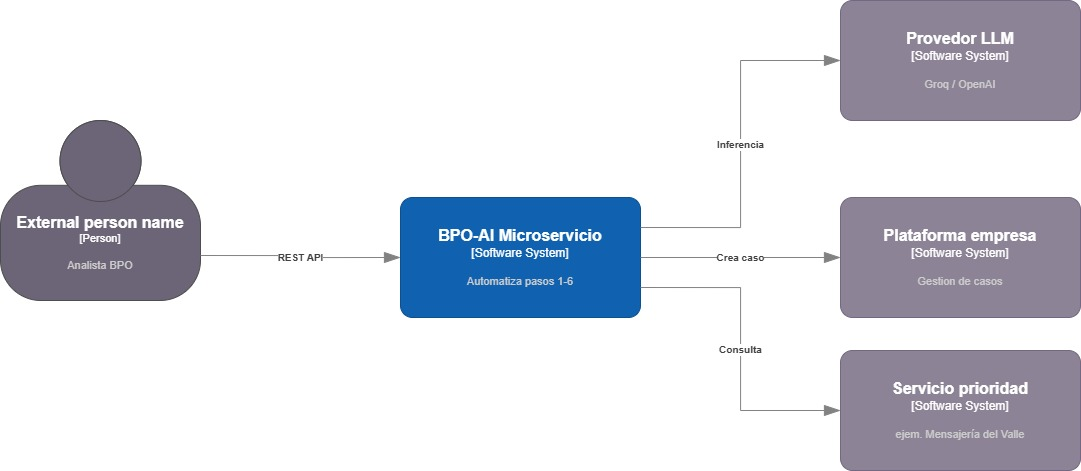
\includegraphics[width=0.82\textwidth]{images/esquema-C4_System.jpg}
\end{center}

El microservicio actúa como punto de entrada único para los analistas BPO. Se integra con tres sistemas externos: el proveedor LLM para inferencia semántica, las plataformas de atención de cada empresa cliente para la creación de casos, y los servicios externos de prioridad que algunos clientes proveen directamente.

\subsection{Nivel 2 --- Contenedores}

\begin{center}
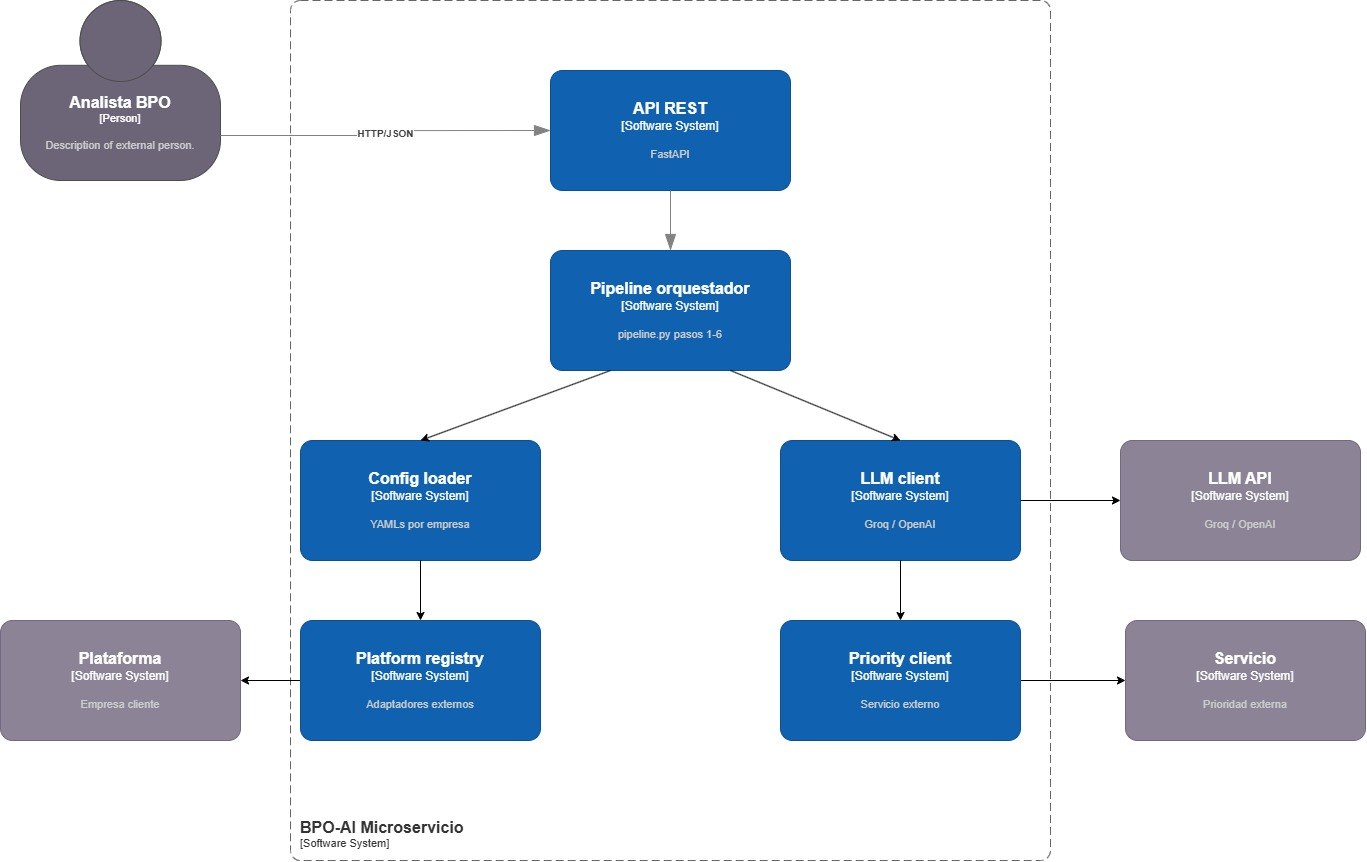
\includegraphics[width=0.88\textwidth]{images/esquema-C4_Container.jpg}
\end{center}

Los contenedores internos están completamente desacoplados entre sí: el pipeline no conoce los detalles del proveedor LLM ni de la plataforma externa. Toda comunicación ocurre a través de interfaces abstractas, lo que permite reemplazar cualquier componente sin afectar al resto.

\subsection{Nivel 3 --- Componentes}

\begin{center}
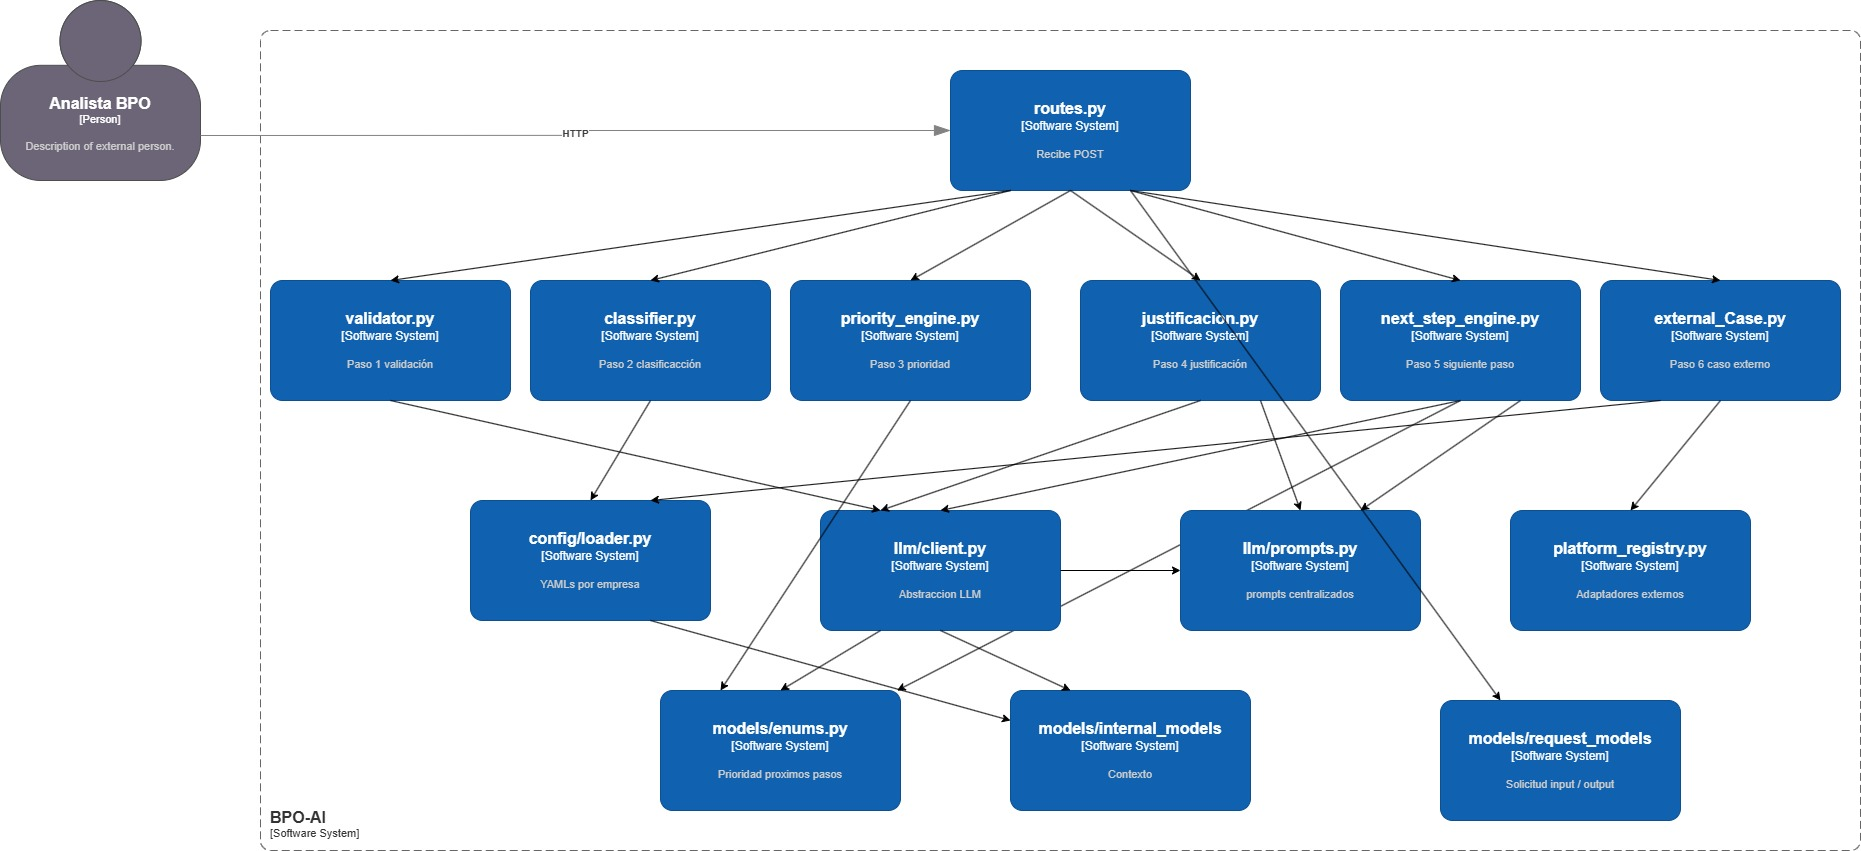
\includegraphics[width=0.92\textwidth]{images/esquema-C4_Component.jpg}
\end{center}

Cada paso del pipeline es un módulo Python independiente con una única responsabilidad. Los módulos de infraestructura compartida (\texttt{llm/client.py}, \texttt{config/loader.py}, \texttt{platform\_registry}) son consumidos por múltiples pasos pero no pertenecen a ninguno, evitando acoplamiento cruzado.

% ── ESCALABILIDAD ────────────────────────────────────────────────────────────
\section{Escalabilidad y Adaptabilidad}

\begin{highlightbox}
\textbf{¿Por qué esta arquitectura soporta el crecimiento?} La variabilidad entre empresas está externalizada en archivos de configuración, no en el código. El código central es agnóstico a los detalles de cada cliente.
\end{highlightbox}

\begin{itemize}[leftmargin=*, itemsep=1pt]
  \item \textbf{Nueva empresa:} Crear un archivo \texttt{app/config/companies/<nombre>.yaml}. Sin cambios en Python.
  \item \textbf{Nueva categoría:} Agregar una línea al YAML de la empresa correspondiente.
  \item \textbf{Cambio de reglas de prioridad:} Modificar las reglas en el YAML. El motor las lee en cada request (con cache).
  \item \textbf{Nueva plataforma externa:} Implementar \texttt{PlataformaExternaBase} y registrar en \texttt{platform\_registry.py}.
  \item \textbf{Nuevo proveedor LLM:} Implementar \texttt{LLMClient} y agregar al factory. Configurable por variable de entorno.
  \item \textbf{Servicio externo de prioridad:} Activar \texttt{prioridad\_externa.activa: true} en el YAML del cliente y configurar la URL como variable de entorno.
  \item \textbf{Mayor volumen:} El diseño stateless de la API permite escalar horizontalmente añadiendo réplicas sin coordinación entre instancias.
\end{itemize}

% ── MANEJO DE ERRORES ─────────────────────────────────────────────────────────
\section{Manejo de Errores}

\begin{itemize}[leftmargin=*, itemsep=1pt]
  \item \textbf{Plataforma externa falla:} El adaptador captura la excepción, registra el error en logs estructurados y retorna el caso con estado \texttt{PENDIENTE\_REINTENTO} y flag \texttt{plataforma\_error: true}. El endpoint \texttt{/solicitudes/health} permite monitorear el estado del servicio. En producción, este flag alimentaría un sistema de alertas (CloudWatch, Datadog).
  \item \textbf{Casos duplicados:} El campo \texttt{solicitud\_id} actúa como idempotency key. En producción se implementaría verificación contra Redis o la base de datos antes de procesar, retornando el resultado cacheado sin reprocesar.
  \item \textbf{Empresa no parametrizada:} El \texttt{config/loader.py} detecta la ausencia del YAML y lanza \texttt{CompanyNotFoundError}, que la capa API convierte en un HTTP 404 con la lista de empresas disponibles, sin que el error llegue al pipeline.
  \item \textbf{LLM no disponible:} Cada paso que usa LLM implementa un fallback determinístico: el validador acepta por longitud mínima, el clasificador asigna ``Otro'', y el justificador genera un texto genérico con los datos disponibles.
\end{itemize}

% ── PERSONALIZACION ──────────────────────────────────────────────────────────
\section{Personalización por Empresa}

El caso de \textbf{Mensajería del Valle} está implementado. En su YAML se configura \texttt{prioridad\_externa.activa: true} y \texttt{endpoint\_env\_var: MENSAJERIA\_VALLE\_PRIORITY\_URL}. El \texttt{priority\_engine.py} detecta esta configuración y llama al microservicio del cliente enviando \texttt{tipo\_documento}, \texttt{numero\_documento} y \texttt{tipo\_solicitud}. Si el servicio externo falla por cualquier razón (timeout, error HTTP, respuesta inválida), el motor hace fallback automático a las reglas locales del YAML, garantizando que el pipeline siempre produce un resultado.

% ── DESPLIEGUE CLOUD ─────────────────────────────────────────────────────────
\section{Propuesta de Despliegue en la Nube (AWS)}

\begin{center}
\small
\begin{tabular}{@{}lll@{}}
\toprule
\textbf{Componente} & \textbf{Servicio AWS} & \textbf{Justificación} \\
\midrule
API REST & API Gateway + ECS Fargate & Escalado automático, sin gestión de servidores \\
Configuración empresas & S3 + Parameter Store & YAMLs versionados, cambios sin redeploy \\
Secretos (API keys) & Secrets Manager & Rotación automática, sin variables en código \\
Cola de solicitudes & SQS & Desacopla ingesta de procesamiento en picos de volumen \\
Logs y métricas & CloudWatch & Alertas sobre \texttt{plataforma\_error}, latencia LLM \\
Cache duplicados & ElastiCache (Redis) & Verificación de \texttt{solicitud\_id} en $<$1ms \\
CI/CD & CodePipeline + ECR & Build, test y deploy automatizados por rama \\
\bottomrule
\end{tabular}
\end{center}



% ── CONCLUSION ───────────────────────────────────────────────────────────────
\section{Conclusión}

La solución entregada automatiza los 6 pasos del proceso BPO con una arquitectura que separa claramente la lógica de negocio (en YAMLs por empresa), la inteligencia artificial (en el cliente LLM), y las integraciones externas (en adaptadores intercambiables). Esta separación garantiza que el crecimiento en número de empresas, categorías o plataformas se gestione mediante configuración, no mediante cambios de código, cumpliendo directamente con los criterios de escalabilidad y adaptabilidad evaluados.

\end{document}